\documentclass[12pt]{scrartcl}
\usepackage{amsmath,amssymb,amsthm}
\usepackage[top=1in, bottom=1in, left=0.8in, right=1in]{geometry}
\usepackage{enumerate}
\usepackage{courier}
\usepackage{hyperref}
\usepackage{multicol}
\usepackage{graphicx}
\renewcommand{\labelenumii}{\roman{enumii}}
\renewcommand{\qedsymbol}{\rule{0.7em}{0.7em}}
\newcommand{\tab}{\phantom{-----}}

\graphicspath{ {Images/} }


\setlength{\columnsep}{2.2em}
\linespread{1}

\title{Comparative Analysis of Artificial Intelligence Techniques for Cancer Diagnostics}
\author{Udai Baiswala - udai, \\ 
Brandon Cui - bcui19, \\ 
Natalie Ng - nng1}
\date{December 16, 2016}
\begin{document}
  \maketitle

  \vspace{-0.3in}
  \rule{\linewidth}{0.4pt}
  \hypersetup{%
    pdfborder = {0 0 0}
}
  
% ##################################################################################
%\begin{multicols*}{2}
    \section{Background}
    In 2000, the National Center for Biotechnology Information established a public repository for the storage of high-throughput biological data called the Gene Expression Omnibus (GEO). To date, scientists have contributed over 4000 datasets with a total of over 2 million samples to GEO. The vast majority of this data was collected via microarrays.
    
    Microarrays are a high-throughput lab-on-a-chip technology that enable measurement of DNA, RNA, and protein levels. In our project, we have narrowed our scope by looking  at datasets which measure cDNA expression levels using a DNA microarray. Since DNA microarrays can measure the expression of at least 20,000 genes simultaneously, they are a powerful tool in biological research. 
    
    To harness the power of DNA microarray data, we need to understand the performance of different analysis techniques on this data format. Typically, scientific labs use non-AI techniques to analyze microarrays. We hope to add AI techniques to the toolkit of analysis pipelines for microarray data. To do so, we must understand the performance of various AI techniques on analyzing microarray data.
    \section{Task Definition}    
    To further narrow the scope of our project, we focus on the application of AI techniques for binary classification problems. After a quick skim of GEO, we notice that the vast majority of the datasets focused on binary classification problems with relation to cancer. Thus, our project focuses on binary classification problems in cancer research. These include classifying tissue between cancerous and benign, distinguishing patients between those that develop relapse and those that remain relapse-free, and diagnosing cancer from circulating blood cells. 
    \subsection{Baseline and Oracle}
Our baseline is an implementation of K Nearest Neighbors. Our oracle is the false positive and false negative rates of current FDA approved cancer screens. Most of these screens range from 5\% to 20\% false positive rates, and 5\% to 10\% false negative rates. 
    \section{Literature Review}
    Current confirms the need for a comparative study of AI techniques in cancer classification problems. In 2006, JA Cruz et. al. report that preliminary machine learning techniques for cancer classification problems improves prediction accuracy by 10-15\% compared to traditional statistical methods. Thus, by gaining a deeper understanding of the benefits and drawbacks of different techniques, we can improve the accuracy of AI techniques by a higher margin.
    
    In 2015, K.Korou et. al. reports that machine learning techniques have been used for binary classification problems related to cancer, but additional validation of these techniques is needed. Our project provides a first step in the validation of such techniques in DNA microarray data.
    \section{Infrastructure}
    We collect our datasets from the Gene Expression Omnibus. These datasets are typically annotated with a chip-specific probe name for a particular gene. We convert these probe names to universal gene names to enable comparison between different datasets. 
    \subsection{Datasets}
    \subsubsection{GSE16449}
    This dataset contains 70 individuals with 34,731 gene expressions each. In addition, the dataset contains information of whether the sample comes from cancerous or benign kidney tissue. We use this dataset for the binary classification problem of cancerous versus benign.
    \subsubsection{GSE13576}
    This dataset contains 196 patients with 55,670 gene expressions each. In addition, the dataset contains information of whether the . We use this dataset for the binary classification problem of cancerous versus benign.
    \subsubsection{ANOTHER ONE}
    fill me in
    \subsection{Normalization}
Microarray data has variation in the amount of each sample inputted into the chip. This leads to a systematic error where one sample has greater expression across all the genes. Thus, we apply a normalization step to each sample. To do this, we sum the expression of the genes for each sample. We then divide each expression by this sum. This scales all the samples to have the same total expression, reducing  noise in the experiment.
    \section{Methods}
	Our methodology consists of running K Nearest Neighbors (KNN) for our baseline and then we implement logistic regression, stochastic gradient descent (SGD), support vector machines (SVMs), Multi-layer neural networks, and Long Short Term Memory (LSTMs).
    
    When training all models, we run 10-fold cross validation. We present the testing error for all such samples. 

	\subsection{Sci-Kit Learn}
    \subsubsection*{5.5.1 K Nearest Neighbors}
    We run 5-NN on our dataset with the KNN package from scikit-learn. The algorithm was ran with a ball tree in order to get around deficiencies in KD-trees and brute force distances. 
    
	\subsubsection*{5.1.2 Logistic Regression}
    For our project we use logistic regression as the baseline for our projection. The logistic regression implementation is performed with the class weight flag turned onto 'balanced'. Thus the weight that each class adds in training is multiplied by the following constant:
    
    $$\frac{\textrm{num samples}}{\textrm{num classInstances}}$$
    
    thus the weights within logistic regression are adjusted inversely proportional to the class frequencies. Overall, this allows for better classification, particularly with our datasets that are biased towards non-cancerous samples. 
    \subsubsection*{5.1.3 Support Vector Machines SVMs}
    We apply SVMs from the sklearn package with the same flag as in logistic regression, where every class was weighted by multiplying it by the constant
    
	$$\frac{\textrm{num samples}}{\textrm{num classInstances}}$$
    
    \subsubsection*{5.1.4 Stochastic Gradient Descent}
    We also use stochastic gradient descent as a means to classify the datasets. Our implementation utilizes hinge loss, an elasticnet penalty, and a balanced class weight. The elasticnet parameter serves to try to optimize the combination of $l1$ and $l2$ as follows:
    
    $$(1-l1ratio)*L2 +l1ratio*L1$$
    
    where the $l1ratio$ is an initialized input constant that defaults to $0.15$ and $L1$ represents the $L1$ norm and $L2$ represents the $L2$ norm. 
    


	\subsection{Tensor Flow}
    fill me in

    \subsection{Preprocessing}
We notice that our data has a high feature to sample ratio. We test the efficacy of a preprocessing step in minimizing overfitting and improving runtime efficiency. Our preprocessing step includes an initial filtration of data to restrict model training to important features that likely have biological relevance. We implement the following two filtration techniques.

    \subsubsection{Differential Expression}
We only include genes that are differentially expressed between the two classifications. We test for significance using a Welch t-test in the sci-py package with a significance cutoff of 0.01. 
    \subsubsection{Fold Change}
We ensure a minimum fold-change of 5. We tested different amounts of fold change and settled on a number that would enable us to retain approximately 10\% of the features in model training.

    \section{Results}
    \subsection{GSE16449: Kidney Cancer Prediction}
    We begin by attempting a binary classification problem between cancerous and benign kidney tissue. 
    \subsubsection{Prediction Accuracy}
    The results below are when running our 5-NN algorithm on the Kidney Cancer dataset (table 1):
   \begin{center}
   \begin{tabular}{c|c|c|c}
   \hline
   & Correctly Predicted & Actual & Percent\\
   \hline
   Cancerous & 18 & 18 & 100\\
   Benign & 52 & 52 & 0\\
   \hline
   \end{tabular}\\
   \vspace{0.1in}
   \textbf{Table 1: 5-NN without Filtration}
    \end{center}
    
    We present the results when running logistic regression on the Kidney Cancer dataset (table 2):
    
    \begin{center}
    \begin{tabular}{c|c|c|c}
    \hline
    & Correctly Predicted & Actual & Percent\\
    \hline
    Cancerous & 16 & 18 & 88.89\\
    Benign & 49 & 52 & 94.23\\
    \hline
    \end{tabular}\\
    \vspace{0.1in}
    \textbf{Table 2: Logistic Regression without Filtration}
    \end{center}
    
    We show the results when running SVMs on the Kidney Cancer dataset (table 3):
    
    \begin{center}
    \begin{tabular}{c|c|c|c}
    \hline
    & Correctly Predicted & Actual & Percent\\
    \hline
    Cancerous & 15 & 18 & 83.3\\
    Benign & 52 & 52 & 100\\
    \hline
    \end{tabular}\\
    \vspace{0.1in}
    \textbf{Table 3: SVM without Filtration}
    \end{center}
    
    We present the results when running 5-NN, Logistic Regression, and SVM on the filtered datasets below:
    
    \begin{center}
    \begin{tabular}{c|c|c|c}
    \hline
    & Correctly Predicted & Actual & Percent\\
    \hline
    Cancerous & 18 & 18 & 100\\
    Benign & 52 & 52 & 0\\
    \hline
    \end{tabular}\\
    \vspace{0.1in}
    \textbf{Table 4: 5-NN with Filtration}
    \end{center}
    
    \begin{center}
    \begin{tabular}{c|c|c|c}
    \hline
    & Correctly Predicted & Actual & Percent\\
    \hline
    Cancerous & 16 & 18 & 88.89\\
    Benign & 52 & 52 & 100\\
    \hline
    \end{tabular}\\
    \vspace{0.1in}
    \textbf{Table 5: Logreg with Filtration}
    \end{center}
    
    \begin{center}
    \begin{tabular}{c|c|c|c}
    \hline
    & Correctly Predicted & Actual & Percent\\
    \hline
    Cancerous & 16 & 18 & 88.89\\
    Benign & 52 & 52 & 100\\
    \hline
    \end{tabular}\\
    \vspace{0.1in}
    \textbf{Table 6: SVM with Filtration}
    \end{center}
    
    
    
    
    \subsubsection{Runtime}
    Due to our preprocessing methods we are able to run all of our methods with a smaller feature set, as a result we are able to see a drastic improvement in runtime. The graph below is the amount of time it takes to load the data and train and test for all 10 folds (figure 1):
    
    \begin{center}
    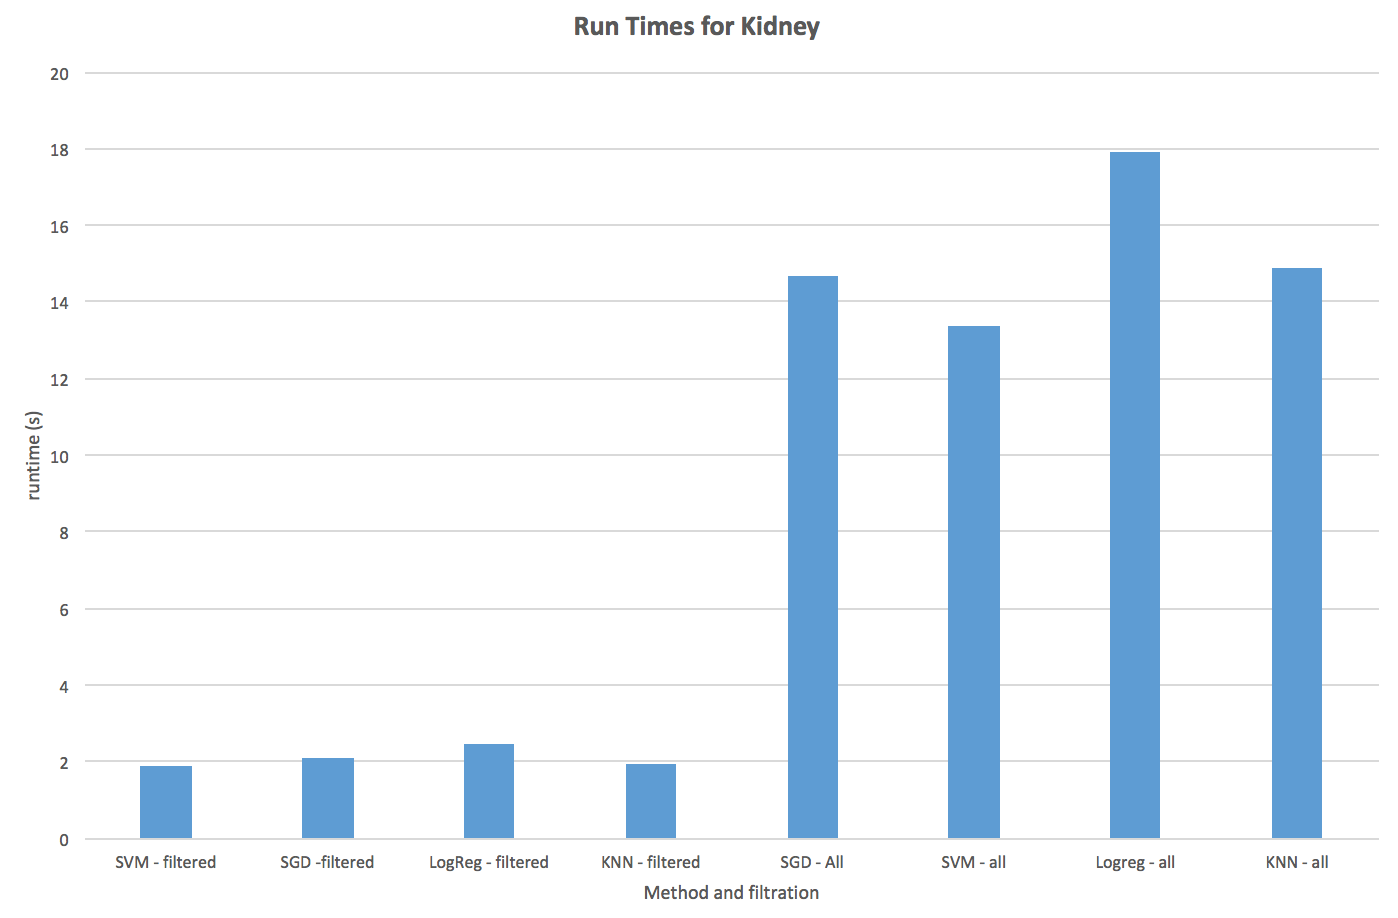
\includegraphics[width = 5in]{runTimeCancer}\\
    \textbf{Figure 1: Runtimes for Different methods on the GSE16449 Dataset}
    \end{center}
    
    \subsubsection{Preliminary Error Analysis}
    We realized that perhaps the classification problem of cancerous versus benign is too trivial. This makes it very difficult to compare the results from different AI techniques, as all techniques will perform reasonably well. We also realize that our dataset does not contain enough samples to do proper training and validation of the model. Thus, in later analysis, we choose harder classification problems with larger datasets.
    
    \subsection{GSE13576: }
    
    \subsubsection{Results}
	We present the classification results for our methodologies below:
    
    \begin{center}
    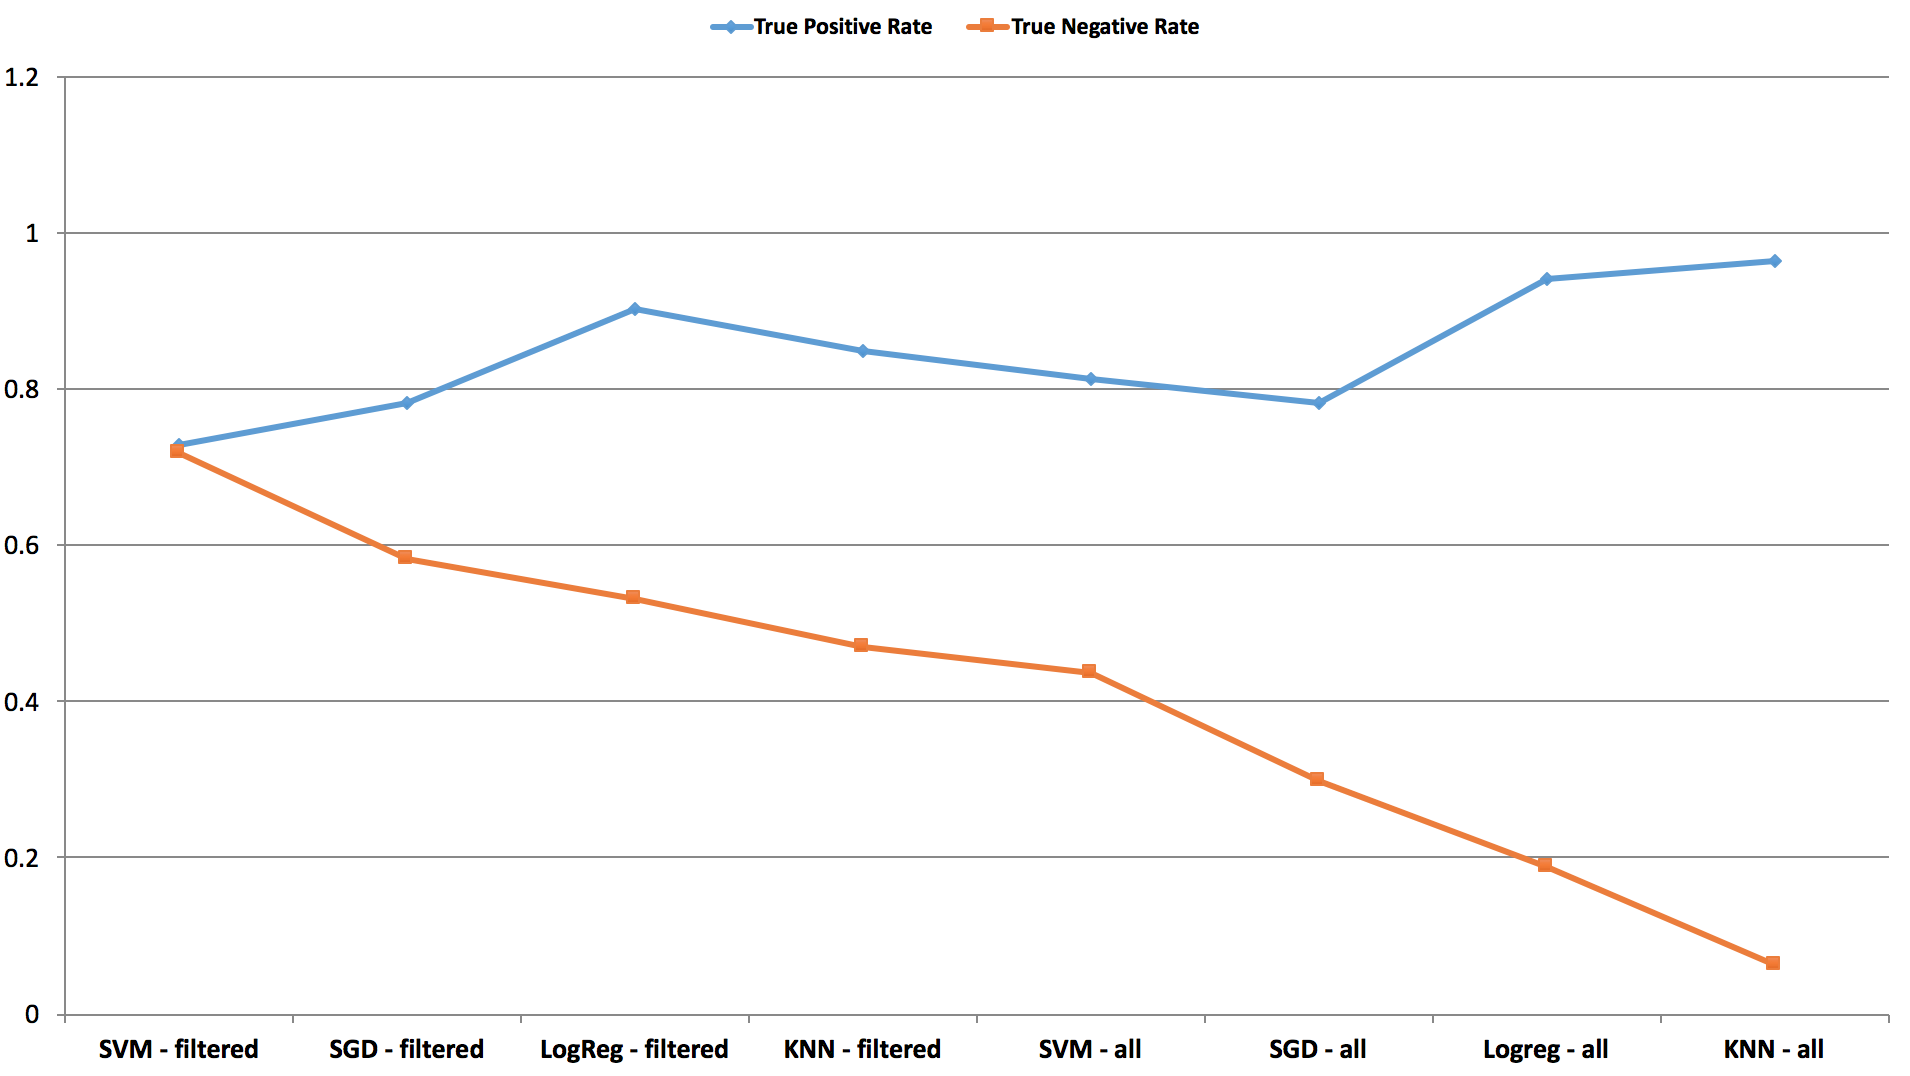
\includegraphics[width = 5in]{classificationResultsRemission}\\
    \textbf{Figure 2:}
    \end{center}
   
  	From the classification results we notice that the filtration of features helps us ensure that the classifier doesn't just classify everything as cancerous. Additionally, we notice that an SVM in both the unfiltered and the filtered case performs best since we want to hit a point where we are accurately able to classify both cancerous and non-cancerous sets of genes.  
   
    \subsubsection{Runtime}
	We show the runtimes for the different algorithms below:
    
    \begin{center}
   	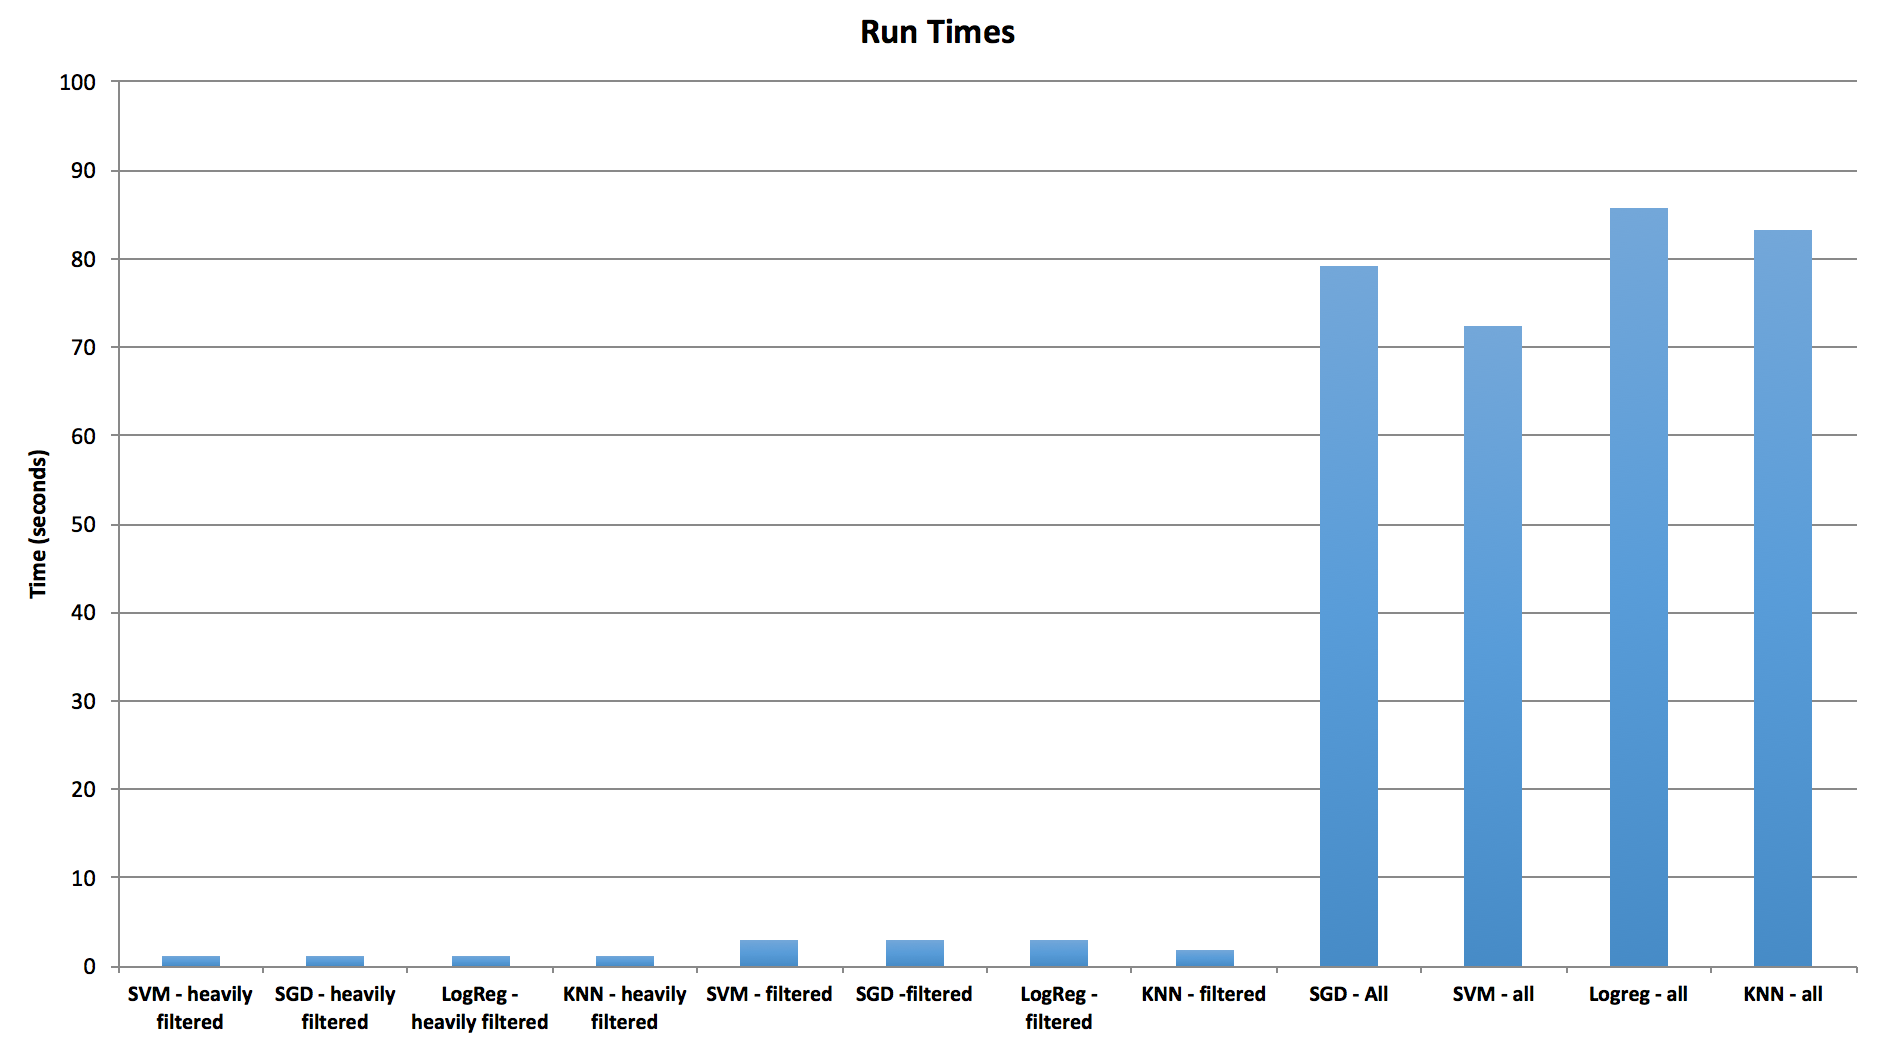
\includegraphics[width = 5in]{runTimeRemission}\\
    \textbf{Figure 2: Runtimes for different methods on the GSE 13576 Dataset}
    \end{center}
    
    We observe that the runtimes for the algorithms are particularly consistent when comparing within the filtered or unfiltered dataset. However, when we compare between the datasets, we notice that the unfiltered dataset performs at over an order of magnitude worse than the filtered dataset
    
    \subsection{Precision and Recall}
    fill me in
    \subsection{Pathway Analysis}
    fill me in

	
    
    \section{Error Analysis}
    fill me in
    
    
    
    \begin{thebibliography}{9}
\bibitem{repmax}
Epley, B. Poundage chart. \textit{Boyd Epley Workout}. Lincoln, NE: Body Enterprises, 1985. p. 86.

\bibitem{jurgens} 
Jurgens, David; McCorriston, James; Rhuts, Derek. 2015. \textit{An Analysis of Exercising Behavior in Online Populations}. McGill University Department of Computer Science. In \textit{Proceedings of ICWSM}.
 
\bibitem{sports} 
United States Dept. of Labor. Bureau of Labor Statistics. \textit{Sports and Exercise}. Web. 14 Dec. 2016. https://www.bls.gov/spotlight/2008/\\sports/.

\bibitem{obnibus}
Barrett, Tanya. "Gene Expression Omnibus (GEO)." \textit{The NCBI Handbook [Internet]}. 2nd Edition. U.S. National Library of Medicine, 2013. Web. 14 Dec. 2016.

\bibitem{cruz}
Cruz, Joseph A., and David S. Wishart. "Applications of Machine Learning in Cancer Prediction and Prognosis." \textit{Cancer Informatics} (2006): 59-77. \textit{US National Library of Medicine}. Web. 14 Dec. 2016.

\bibitem{kourou}
Kourou, Konstantina, Themis Exarchos, and Konstantinos Exarchos. "Machine Learning Applications in Cancer Prognosis and Prediction." \textit{Computational and Structural Biotechnology Journal} 13 (2015): 8-17. Web. 14 Dec. 2016.

\end{thebibliography}
    
%\end{multicols*}
\end{document}
